\documentclass[11pt]{article}
\usepackage[margin=1in]{geometry}
\usepackage{../../styles/isaiah}
\usepackage{../../styles/components/threeBoxGrid}

\begin{document}

% Overview of Isaiah 1-12 Chiastic Structure
\isaiahChiasticOverview{5}

\newpage

% Isaiah Context Grid
\threeBoxGrid{1}{Isaiah 9:8-10:34}{
    \textbf{\large Isaiah 9:8-21}

    \textit{Anger not Turned \\Away from Israel}
}{
    \textbf{\large Isaiah 10:1-4}

    \textit{Woe to Israel \& Anger \\not Turned Away}
}{
    \textbf{\large Isaiah 10:5-34}

    \textit{Woes and Therefores \\to Assyria}
}

% Overview of Isaiah 9:8-10:27
\begin{overview}{Isaiah 9:8-9:21 — Overview}

\overviewsection[0]{%
\textbf{Verses 8-12: Nations against Israel}
}

\overviewsection[1]{%
\textbf{Verses 13-17: Israel's Leaders against Poor}
}

\overviewsection[0]{%
\textbf{Verses 18-21: Israel against Itself}
}

\end{overview}
\newpage

% Verses 8-12 - Nations against Israel
\begin{biblicaloutline}[Isaiah 9:8-12]

    \begin{versesection}{2em}
        \poetryline{\versenum{8} The Lord has sent a \sectionwordfootnote{word}{Septuigent – "plague/death"} against Jacob,}
        \poetryline{and it will fall on Israel;}
        \poetryline{\versenum{9} and all the people will know,}
        \poetryline{\highlightyellow{Ephraim} and the inhabitants of Samaria,}
        \poetryline{who say in pride and in arrogance of heart:}
        \poetryline{\versenum{10} "The bricks have fallen,}
        \poetryline{but we will build with dressed stones;}
        \poetryline{the sycamores have been cut down,}
        \poetryline{but we will put cedars in their place."}
        \poetryline{\versenum{11} But the LORD raises the adversaries of Rezin against him,}
        \poetryline{and stirs up his enemies.}
        \poetryline{\versenum{12} The Syrians on the east and the \sectionwordfootnote{Philistines on the west}{C.f. Amos 1:6 – Could be figurative or they could've been involved in capturing the fleeing Israelites during Assyrian invasion}}
        \poetryline{\highlightblue{devour} Israel with \highlightblue{open mouth}.}
        \poetryline{\highlightorange{For all this his anger has not turned away,}}
        \poetryline{\highlightorange{and his hand is stretched out still.}}
    \end{versesection}

\end{biblicaloutline}

\vspace{3em}

% Verses 13-17 - Israel's Leaders against Poor
\begin{biblicaloutline}[Isaiah 9:13-17]

    \begin{versesection}{2em}
        \poetryline{\versenum{13} The people did not turn to him who struck them,}
        \poetryline{nor inquire of the LORD of hosts.}
        \poetryline{\versenum{14} So the LORD cut off from Israel head and tail,}
        \poetryline{palm branch and reed in one day—}
        \poetryline{\versenum{15} the elder and honored man is the head,}
        \poetryline{and the prophet who teaches lies is the tail;}
        \poetryline{\versenum{16} for those who guide this people have been leading them astray,}
        \poetryline{and those who are guided by them are \highlightblue{swallowed up}.}
        \poetryline{\versenum{17} Therefore the Lord does not rejoice over their young men,}
        \poetryline{and has no compassion on their \highlightpurple{fatherless} and \highlightpurple{widows};}
        \poetryline{for everyone is godless and an evildoer,}
        \poetryline{and every \highlightblue{mouth} speaks folly.}
        \poetryline{\highlightorange{For all this his anger has not turned away,}}
        \poetryline{\highlightorange{and his hand is stretched out still.}}
    \end{versesection}

\end{biblicaloutline}

\vspace{3em}

% Verses 18-21 - Israel against Itself
\begin{biblicaloutline}[Isaiah 9:18-21]

    \begin{versesection}{2em}
        \poetryline{\versenum{18} For wickedness burns like a \highlightred{fire};}
        \poetryline{it \highlightblue{devours} briers and thorns;}
        \poetryline{it kindles the thickets of the forest,}
        \poetryline{and they roll upward in a column of smoke.}
        \poetryline{\versenum{19} Through the wrath of the LORD of hosts}
        \poetryline{the land is scorched,}
        \poetryline{and the people are like fuel for the \highlightred{fire};}
        \poetryline{no one spares another.}
        \poetryline{\versenum{20} They slice meat on the right, but are still hungry,}
        \poetryline{and they \highlightblue{devour} on the left, but are not satisfied;}
        \poetryline{each \highlightblue{devours} the flesh of his own \sectionwordfootnote{arm}{Septuigent – "Brother"; Could also be interpreted "seed"}:}
        \poetryline{\versenum{21} Manasseh \highlightblue{devours} \highlightyellow{Ephraim}, and \highlightyellow{Ephraim} Manasseh;}
        \poetryline{and together they are against Judah.}
        \poetryline{\highlightorange{For all this his anger has not turned away,}}
        \poetryline{\highlightorange{and his hand is stretched out still.}}
    \end{versesection}

\end{biblicaloutline}

\vspace{3em}
{\large\bfseries "Hand Still Stretched Out"}
\vspace{1em}

[Placeholder: Read Ex. 6:6 and Deut 4:34. The stretched out hand can be the power to save or the power to judge]

\vspace{3em}
{\large\bfseries "Devoured"}
\vspace{1em}

[Placeholder: Seeing the repeated phrases around eating/swallowing up, we can see what Israel's leaders are doing to their vulnerable is put on analogy to what the Syrians and Philistines are doing to Israel. This gets shown more explicitly in the final section of this passage.]

\vspace{3em}
{\large\bfseries God has no compassion on Poor?}
\vspace{1em}

[Placeholder: The opposite of taking care of them is teaching lies and leading astray. Even those who are supposed to be cared for are led to moral corruption by the leaders. Kind of like how the prosperity gospel of today feeds on the vulnerable and leads them away from the truth.]

\vspace{3em}
{\large\bfseries Who's Doing This?}
\vspace{1em}

[Placeholder: In v18-21 we see a pattern that started all the way back in the early chapters of Genesis: God's wrath being evidenced as handing people over to their own desires (we can cross reference that passage in the flood story that says this).]

\vspace{3em}
{\large\bfseries Bricks, Stones, Sycamores, and Cedars}
\vspace{1em}

[Placeholder: Add analysis of the arrogant response in v9-10]

\vspace{1em}
\begin{center}
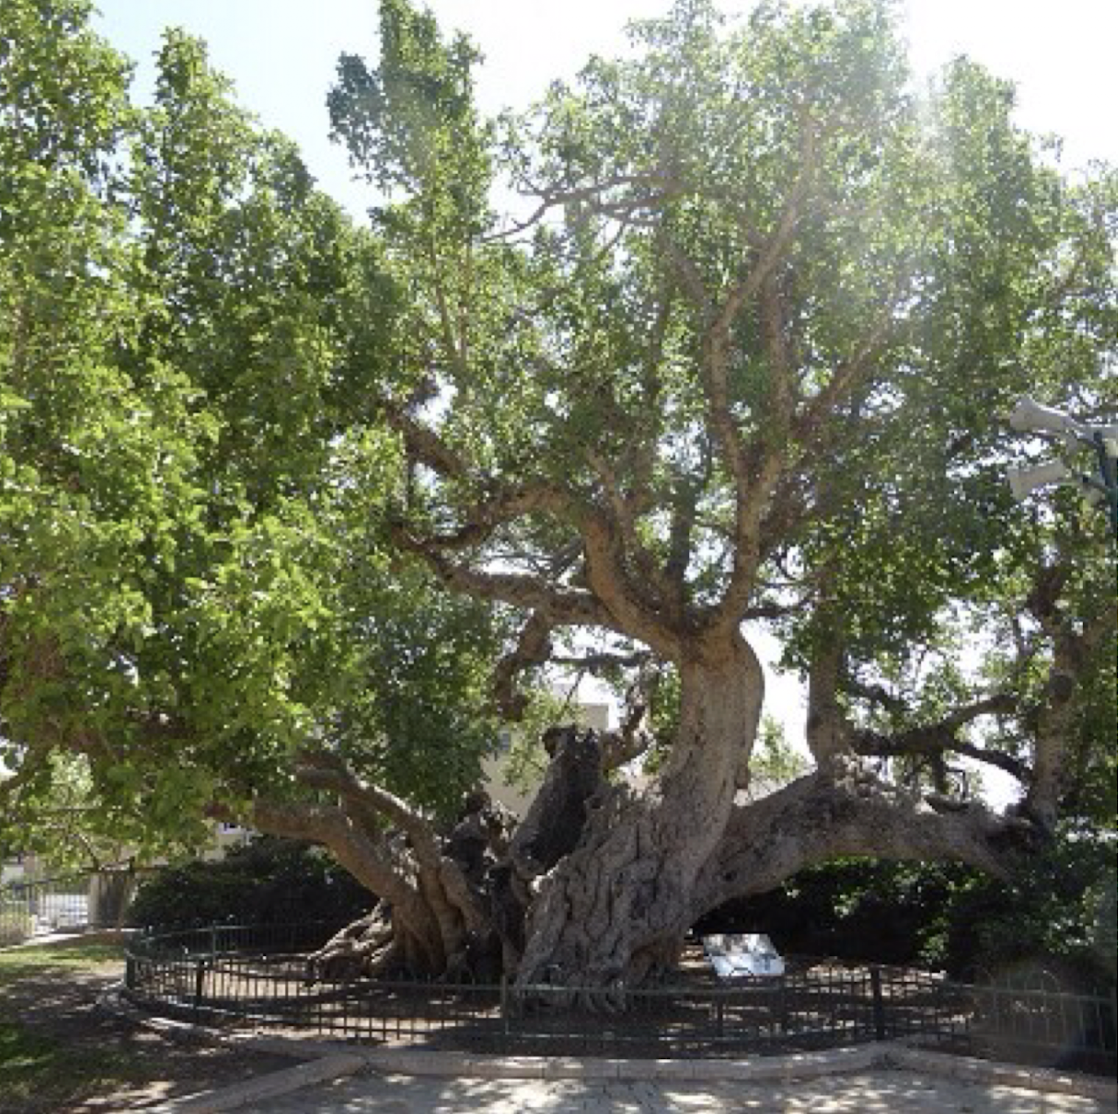
\includegraphics[width=0.45\textwidth]{sycamore.png}
\hspace{0.05\textwidth}
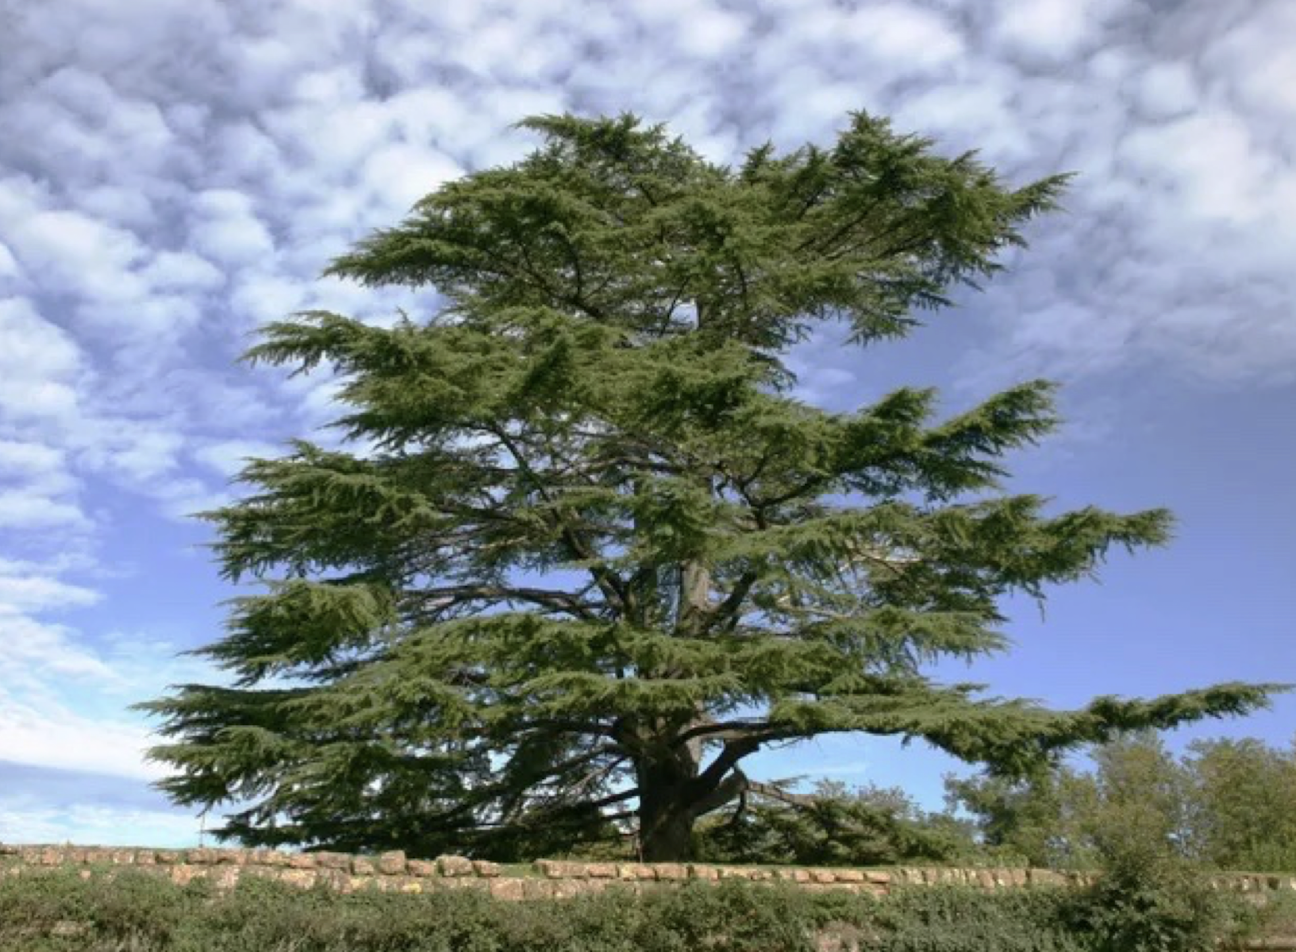
\includegraphics[width=0.45\textwidth]{lebanon-cedar.png}
\end{center}
\vspace{1em}

\begin{center}
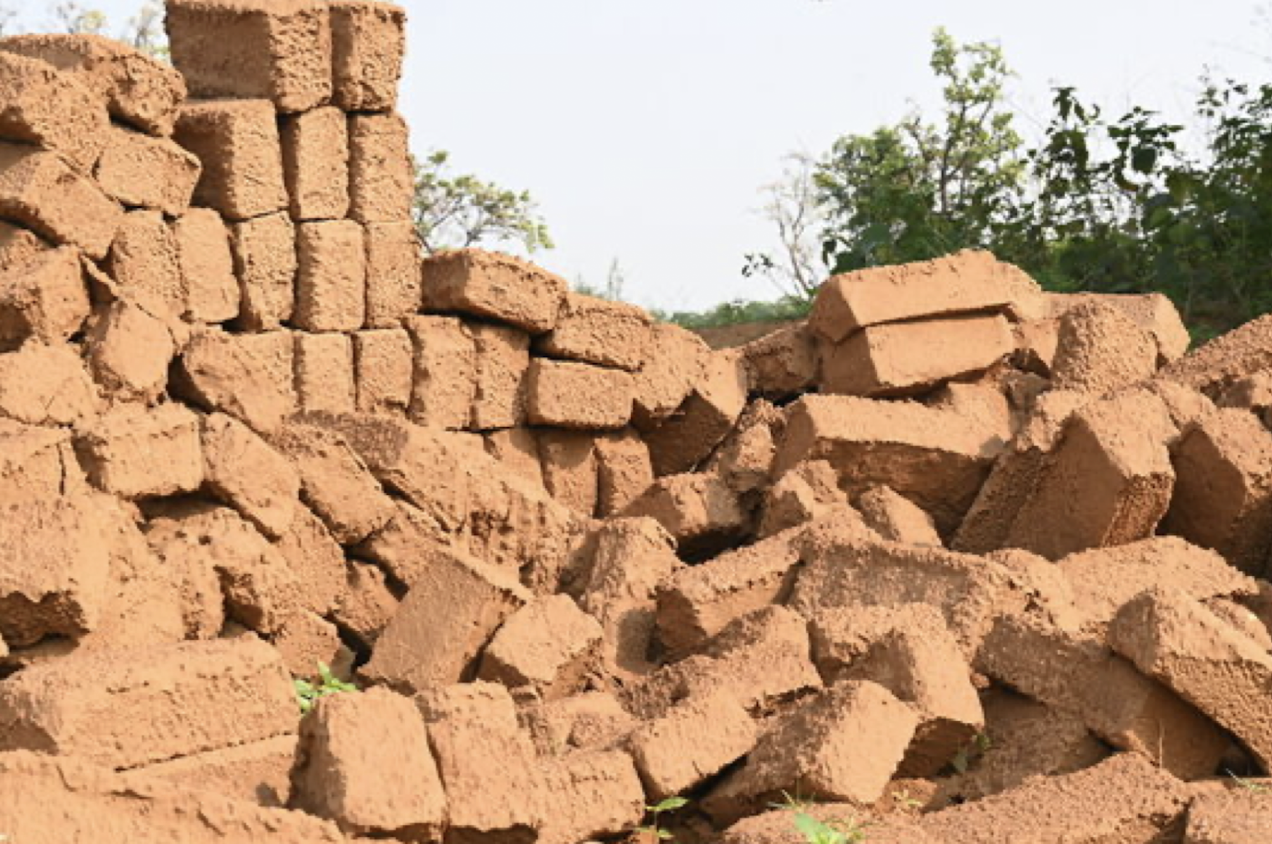
\includegraphics[width=0.45\textwidth]{mud-bricks.png}
\hspace{0.05\textwidth}
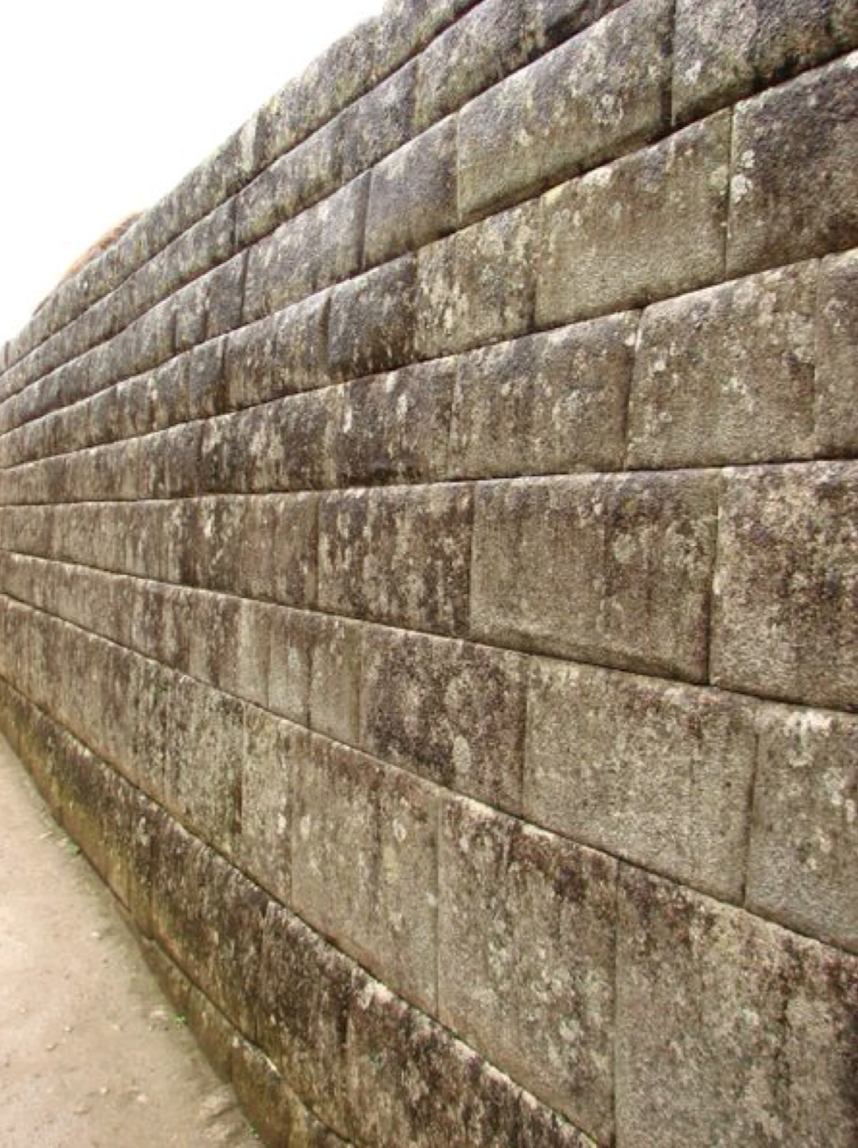
\includegraphics[width=0.45\textwidth]{ashlar-stones.png}
\end{center}
\vspace{1em}

\end{document}
